\chapter{实验结果}

\section{输入语句的测试案例}

首先我们聚焦于语义搜索的结果,我们可以看见,搜索“温柔”,得到的前20个艺术品为:

\footnotesize
“ 2009年作 你的温柔 布面 油画 ”;
“ 2009年作 温柔的坚持 布面 油画 ”;
“ 1997年作 温柔的风 布面 油画 ”;
“ 1993年作 温柔的光 布面 油画 ”;
“ 2007年作 下午温柔的阳光 布面油画 ”;
“ 2003年作 温柔的光 布面油彩 ”;
“ 2003年作 温柔的光 布面 油彩 ”;
“ 1989年作 温柔的音乐 油彩画布 镜框 ”;
“ 1997年作 温柔的沉思 油彩 画布 ”;
“ 1992年作 温柔情人 压克力纸本 ”;
“ 1992年作 温柔情人 压克力 纸本 ”;
“ 2013年作 夜色温柔 布面油画 ”;
“ 2010年作 夜色温柔 布面 油画 ”;
“ 温柔地杀我 油画 画布 ”;
“ 2004年作 温柔地杀我 版画 ”;
“ 2002年作 温柔地杀我 布面 油画 ”;
“ 2010年作 优雅的女孩 布面 油画 ”;
“ 2009年作 你的柔情 布面 油彩 ”;
“ 灿烂的朝阳照在秋日收……”;
“ 2009年作 你的柔情 布面 油画 ”。

\normalsize
可以看到,非常明显的,和“温柔”相关的艺术品题目被首先搜索了出来,“xxx年作”“我的”这样的单词由于在总体文本中高频出现,故而权重低,引起的偏移很低。最后一个题目中带有“温柔”的作品很有意思,叫做“温柔地杀我”,显然,作者在命名这样一个名字的时候使用了对比的手法,“杀”之类的词语的词向量显然和“温柔”方向不同,以至于使得这个题目的句向量偏移到更远的地方,成为了题目中带有“温柔”的作品中排在最后的作品。而更应当注意的是,当题目中带有“温柔”的作品都被搜索出来之后,从第17个艺术品开始,我们可以发现题目中不再出现“温柔”这个单词,而出现了“优雅的女孩”,“柔情”等从“温柔”的语义延伸的词语,这更直接的说明word2vec发挥了它的优势,在向量化的过程中“温柔”和“柔情”等词的词向量距离很近。

如果加入更多的干扰信息,输入“我想要温柔的柔和的感觉”,得到的前20个艺术品为:

\footnotesize
“ 第二年,我去了北京,在那…… ”;
“ 受马蒂斯的影响,闫平的画…… ”;
“ 杨飞云的艺术真正打动人的,…… ”;
“ 这种自觉的留白和色彩的简…… ”;
“ 居于大地的当代生存者正在描…… ”;
“ 20世纪80年代以来,他从写实……”;
“ 1993年作 温柔的光 布面 油画 ”;
“ 2003年作 温柔的光 布面油彩 ”;
“ 2003年作 温柔的光 布面 油彩 ”;
“ 2007年作 下午温柔的阳光 布面油画 ”;
“ 1989年作 温柔的音乐 油彩画布 镜框 ”;
“ 刘海粟这个时期的作品有一种……”;
“ 1982年我毕业后被留校任教,…… ”;
“ 具象和抽象迭合构成的"古典"作……”;
“ 他的深度绘画表现和塑造的是……”;
“ 毛时安评论说:“俞晓夫是很聪明…… ”;
“ 2009年作 温柔的坚持 布面 油画 ”;
“ 创作于1995年的作品《抽象》…… ”;
“ 《小演员》画面中少女肌肤所充溢……”。

\normalsize
(在这里由于某些文本过长,没有全部显示,可以在附录中查找到实验结果的所有结果。)受到干扰信息的影响,其中大多数都是带有长长的描述的艺术品文本,在数据库中出现这样一类的文本,题目为长长的描述,图片的url则为空缺。之前我已经进行过数据清理(见第二章),在这里意识到数据清理还需要补充,由于本系统聚焦于色彩方案提取,所以我去除了这些没有图片资料的艺术品。

\footnotesize
“ 1993年作 温柔的光 布面 油画 ”;
“ 2003年作 温柔的光 布面油彩 ”;
“ 2003年作 温柔的光 布面 油彩 ”;
“ 2007年作 下午温柔的阳光 布面油画 ”;
“ 1989年作 温柔的音乐 油彩画布 镜框 ”;
“ 2009年作 温柔的坚持 布面 油画 ”。

\normalsize
除了这些本身就没有题目和图片信息的艺术品之外,其他的艺术品文本都是围绕“温柔、柔和”,可以达成使用者的目标。




让我们继续来看的色彩方案和上色结果,输入“我想要温柔的柔和的感觉”,得到的效果图如图~\ref{figure:温柔}。

\begin{figure}[!htbp]
\centering
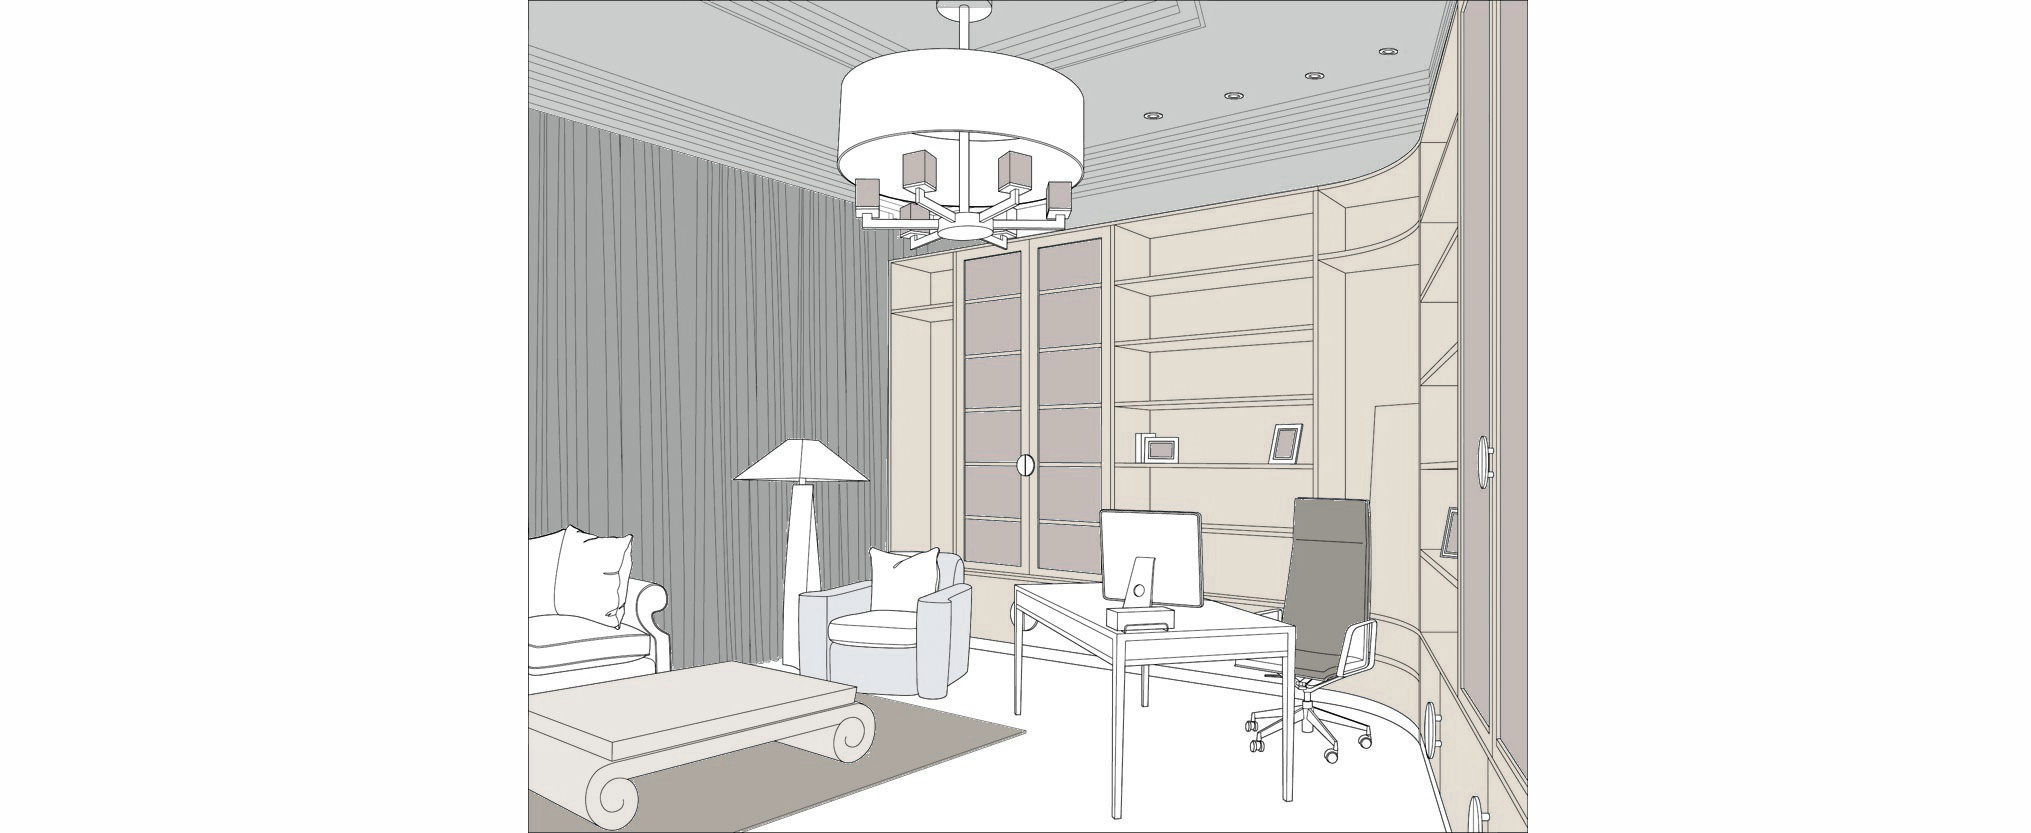
\includegraphics[width=\linewidth,keepaspectratio]{data/chapter-4/温柔.jpg}
\caption{输入“我想要温柔的柔和的感觉”}
\label{figure:温柔}
\end{figure}

输入“温柔的女性化的感觉”,作为人类的理解,这句话与上一句话的区别为,上一句话主要是“温柔/柔和”,这句话不仅强调“温柔”还强调“女性化”。输入“温柔的女性”,相当于对系统提出了两个要求,要求输出的结果既符合“温柔”又符合“女性”,得到的前20个艺术品为:

\footnotesize
“ 2009年作 温柔的坚持 布面 油画 ”;
“ 2009年作 你的温柔 布面 油画 ”;
“ 新女性 布面 油画 ”;
“ 新女性 布面 油画 ”;
“ 1993年作 温柔的光 布面 油画 ”;
“ 1997年作 温柔的风 布面 油画 ”;
“ 2007年作 下午温柔的阳光 布面油画 ”;
“ 2003年作 温柔的光 布面 油彩 ”;
“ 2003年作 温柔的光 布面油彩 ”;
“ 1989年作 温柔的音乐 油彩画布 镜框 ”;
“ 2006年作 新女性 布面油画 ”;
“ 2003年作 新女性 布面油画 ”;
“ 2003年作 当代女性 布面 油画 ”;
“ 1997年作 温柔的沉思 油彩 画布 ”;
“ 2002年作 新女性 布面油画 ”;
“ 2011年作 戴银饰的苗族女人 布面 油画 ”;
“ 2006年作 现代女性 油画 画布 ”;
“ 2007年作 美丽上海—她们的眼睛 布面 油画 ”;
“ 2010年作 优雅的女孩 布面 油画 ”;
“ 2013年作 优雅女人 布面油画 ”;

\normalsize
可以看到搜索结果其实分为靠近“温柔”的和靠近“女性”的,在“温柔”和“女性”结合的程度上显得不是很好,这样的结果收到数据库的限制,因为数据库中艺术品的文本包括“温柔”和“女性”两个含义的(并非必须这两个词)不常见。这是这个系统的一个限制,即数据库中的艺术品不能囊括所有的感受,并且即使艺术品中包含的信息和感受很多,艺术品文本包含的信息一定比艺术品本身少,艺术品文本描述的并不一定是艺术品的色彩风格。解决这个问题采用了交互设计的办法,即搜索最为匹配的前10个结果,对其中随机的一个提取颜色产生色彩方案。这样用户可以通过不改变输入文本,再次搜索,系统就会另外随机选择一件,直到用户得到满意的方案;用户也可以手动打开10个色彩方案手动选择。

对于配色方案我的期望是,比上图有更多的女性特质的方案,也许整体是偏粉红色或有其他符合女性特征的特点。而系统运行的结果如图~\ref{figure:温柔女},图~\ref{figure:温柔女2},是符合预期的。

\begin{figure}[!htbp]
\centering
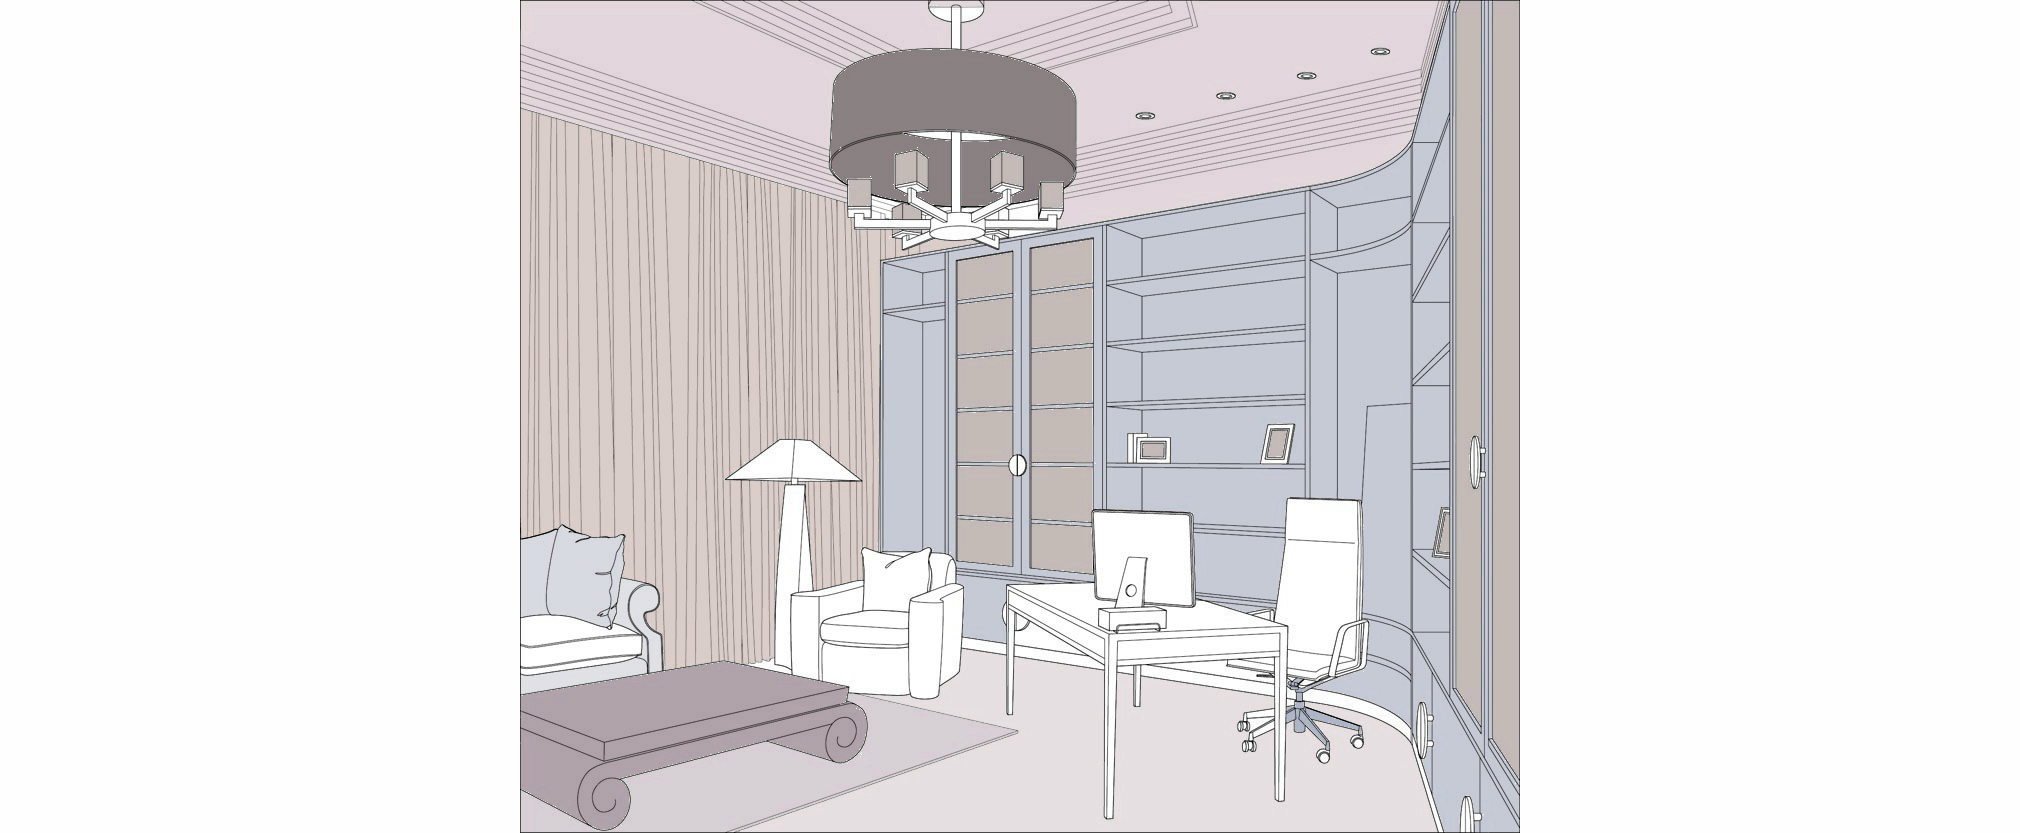
\includegraphics[width=\linewidth,keepaspectratio]{data/chapter-4/温柔女性.jpg}
\caption{输入“温柔的女性化的感觉”}
\label{figure:温柔女}
\end{figure}

\begin{figure}[!htbp]
\centering
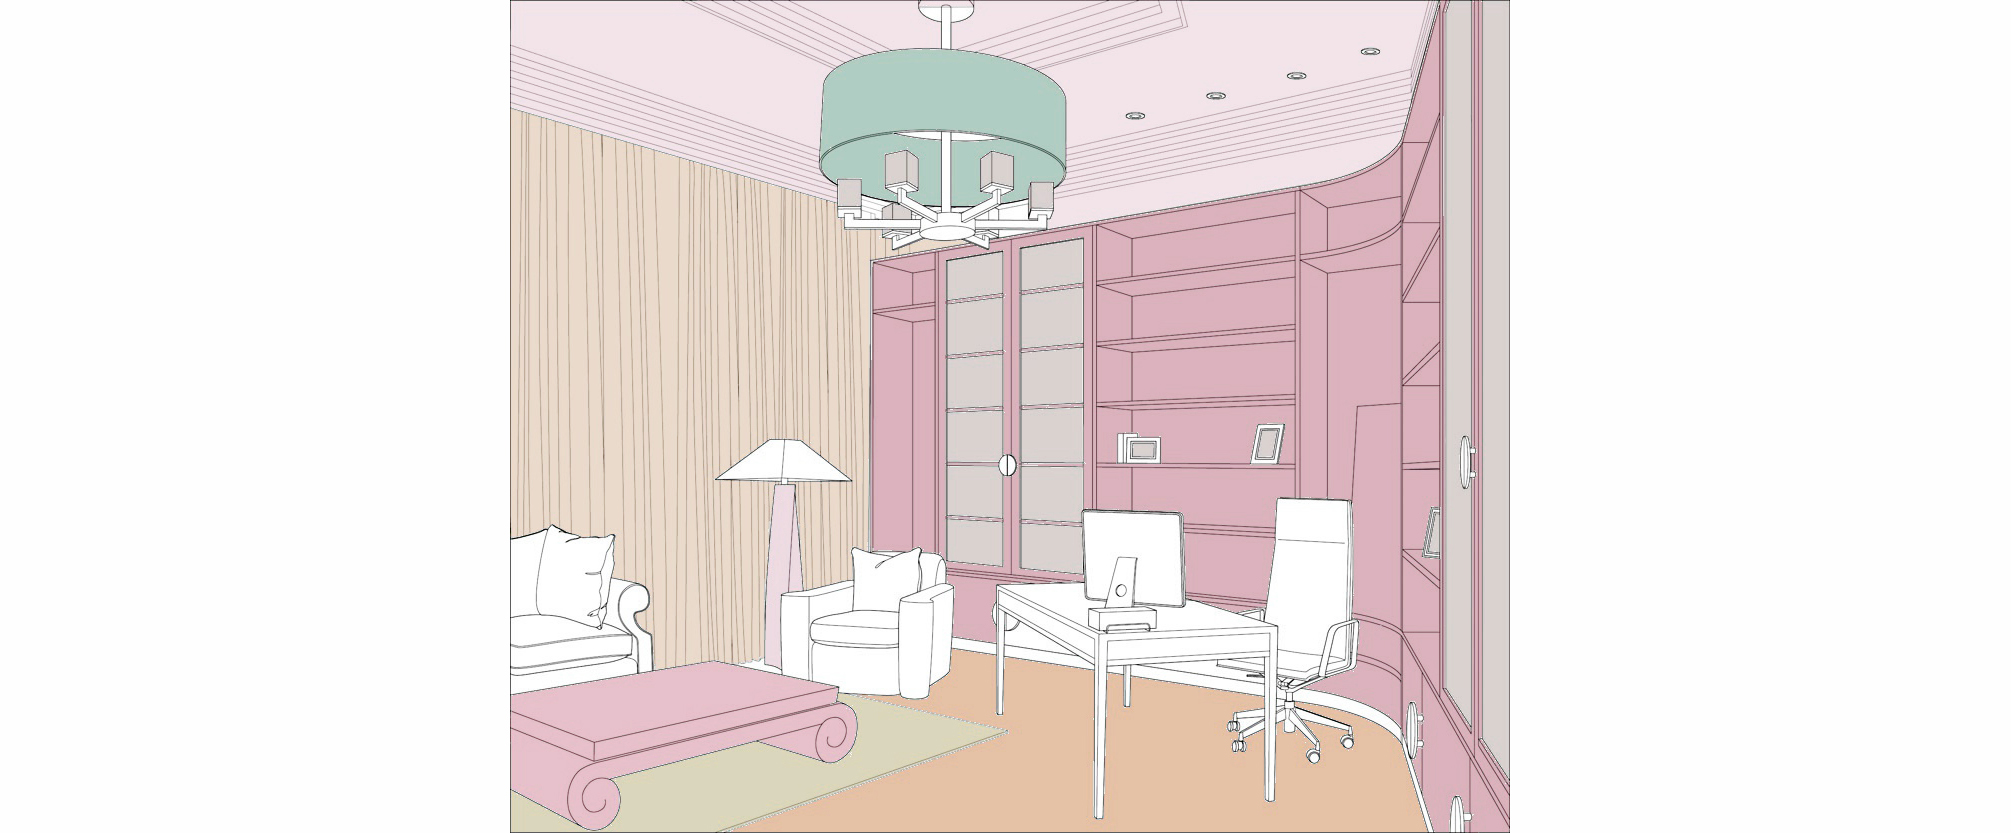
\includegraphics[width=\linewidth,keepaspectratio]{data/chapter-4/温柔女性2.jpg}
\caption{输入“温柔的女性化的感觉”}
\label{figure:温柔女2}
\end{figure}

那么如果输入“冷静的男性”。得到的结果是让人不满意的:

\footnotesize“ 新女性 布面 油画 ”;
“ 新女性 布面 油画 ”;
“ 2004年作 冷静 油彩 画布 ”;
“ 喻红在日常存在中寻找到一种诗意…… ”;
“ 2006年作 新女性 布面油画 ”;
“ 陈擎耀历年来的数字合成影像作品……”;
“ 我历年来的数字合成影像作品,皆……”;
“ 刘海粟是要强的人,有强烈的自我…… ”;
“ 1989年北京的现代艺术大展标志……”;
“ 刘海粟这个时期的作品有一种较……”;
“ 受马蒂斯的影响,闫平的画面中,表……”;
“ 2011年作 戴银饰的苗族女人 布面 油画 ”;
“ 不过站在美术史的角度上来看,从……”;
“ 居于大地的当代生存者正在描摹……”;
“ 2006年作 现代女性 油画 画布 ”;
“ 最显著的是911事件后,城市、霸权……”;
“ 《男男女女》创作于2006年,是刘……”;
“ 2003年作 当代女性 布面 油画 ”;
“ 2003年作 新女性 布面油画 ”;
“ 1999年作 理智与情感 油画 画布 ”;

\normalsize
在这里就发生了一个问题,想要男性化的风格得到的搜索结果全是女性。这是由于word embedding的词向量本身的性质。由于词向量基于上下文预测,所以最为相似的单词并非语义上最相似,而是用法上最相似的单词,比如“男性”和“女性”往往用在相同的上下文环境中,而“男性”和“男人”相对用在相同上下文环境中的程度更小一些。如果我们适应一下这个系统,输入“冷静的男人”那么就会得到这样的搜索结果:

\footnotesize
“ 2004年作 冷静 油彩 画布 ”;
“ 1995年作 大眼睛男人 布面 油画 ”;
“ 2011年作 戴银饰的苗族女人 布面 油画 ”;
“ 2007年作 红色男人 布面油画 ”;
“ 2006年作 男人像 油画 ”;
“ 清 男人像 纸本油画 ”;
“ 男人像 油画 画布 ”;
“ 男人像 油画 画布 ”;
“ 2008年作 男人 布面 油画 ”;
“ 两个男人 纸本 油画 ”;
“ 2005年作 男人肖像 布面油画 ”;
“ 男人的故事 ”;
“ 男人 布面 油画 ”;
“ 男人 布面 油画 ”;
“ 2007年作 红色男人 油彩 布面 ”;
“ 1999年作 男人与马 布面 油画 ”;
“ 喻红在日常存在中寻找到一种诗意。她……”;
“ 1997年作 同志系列:男人 布面 油画 ”;
“ 2006年作 红色男人像 油彩 画布 ”;
“ 2001年作 男人·女人 布面 油画 ”;
\normalsize

如图~\ref{figure:冷静的男人},比起“温柔”来看的确显得更加沉稳厚重。

\begin{figure}[!htbp]
\centering
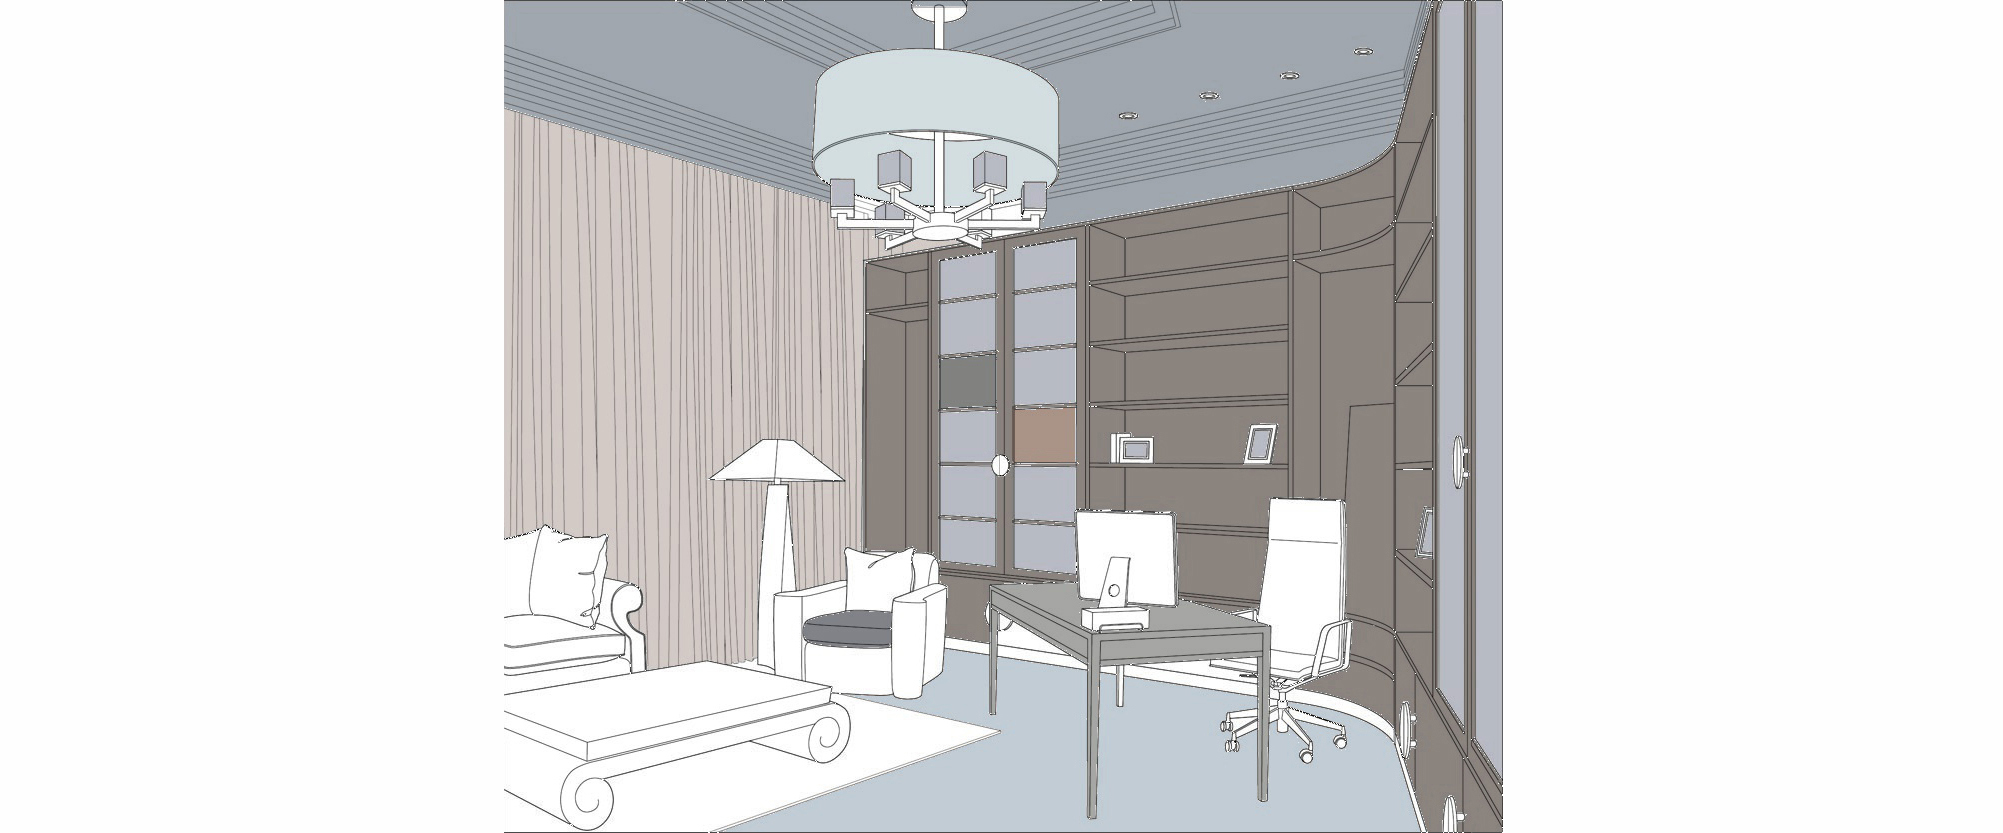
\includegraphics[width=\linewidth,keepaspectratio]{data/chapter-4/冷静的男性}
\caption{输入“冷静的男人”}
\label{figure:冷静的男人}
\end{figure}

输入“快乐的儿童”,输入“快乐的儿童”搜到的艺术品有:

\footnotesize
“ 1997年作 快乐的儿童 第9号 油画 画布 ”;
“ 2013年作 快乐的孩子们 布面油画 ”;
“ 新中国的儿童 (一张) 纸本 ”;
“ 儿童 布面油画 ”;
“ 儿童 油画 ”;
“ 2004年作 儿童时代 油画画布 ”;
“ 快乐1 油画 ”;
“ 1997年作 为小孩快乐 油画画布 ”;
“ 2001年作 快乐世界 布面油画 ”;
“ 少女与儿童 布面 油画 ”;
“ 2005年作 快乐在一起,2号 油画画布 ”;
“ 快乐的童年 布面油画 ”;
“ 1999年作 快乐的红色 油画 画布 ”;
“ 1992年作 快乐 油画画布 ”;
“ 游戏的儿童 布面油画 ”;
“ 快乐的童年 油画画布 ”;
“ 威尼斯的快乐 ”;
“ 2002年作 游戏的儿童9号 油画画布 ”;
“ 2002年作 游戏的儿童8号 油画画布 ”;
“ 2005年作 快乐组合 布面油画 ”。

\normalsize
显示程序完全可以抽象出“儿童”和“小孩”、“孩子”的相似性。得到的图~\ref{figure:儿童2}的色彩方案,虽然使用的效果图线稿是一个书房,但是也能看出符合方案儿童房的配色。

\begin{figure}[!htbp]
\centering
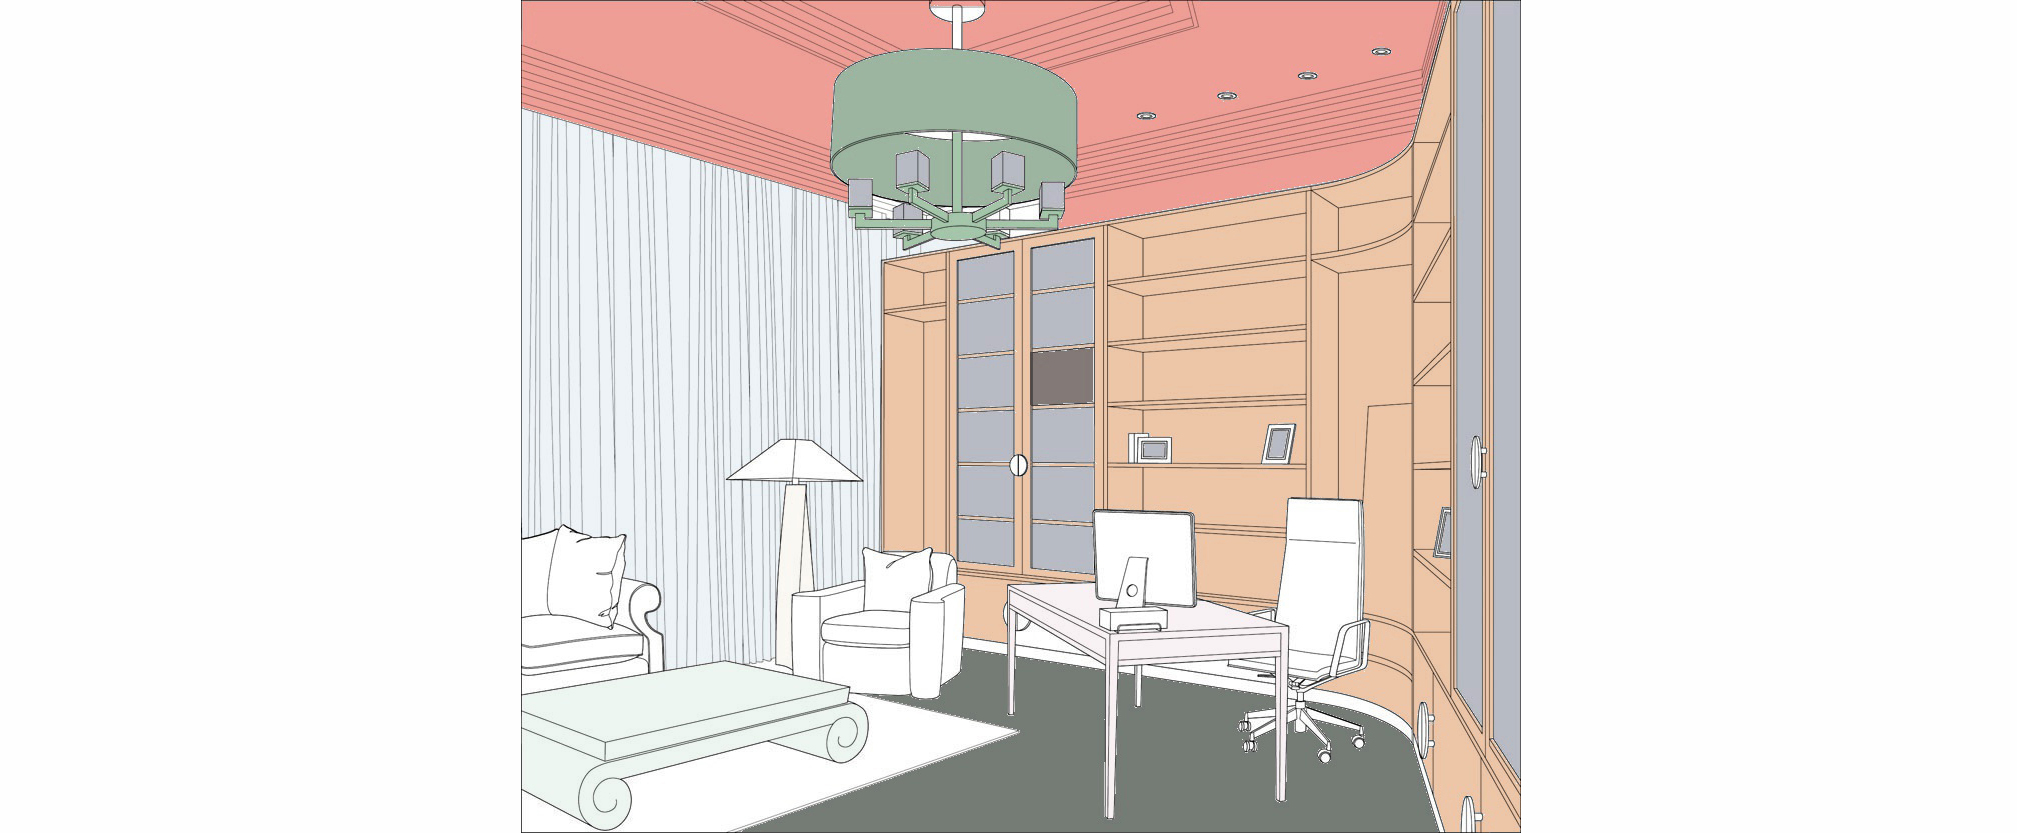
\includegraphics[width=\linewidth,keepaspectratio]{data/chapter-4/快乐儿童2.jpg}
\caption{输入“快乐的儿童”}
\label{figure:儿童2}
\end{figure}

\begin{figure}[!htbp]
\centering
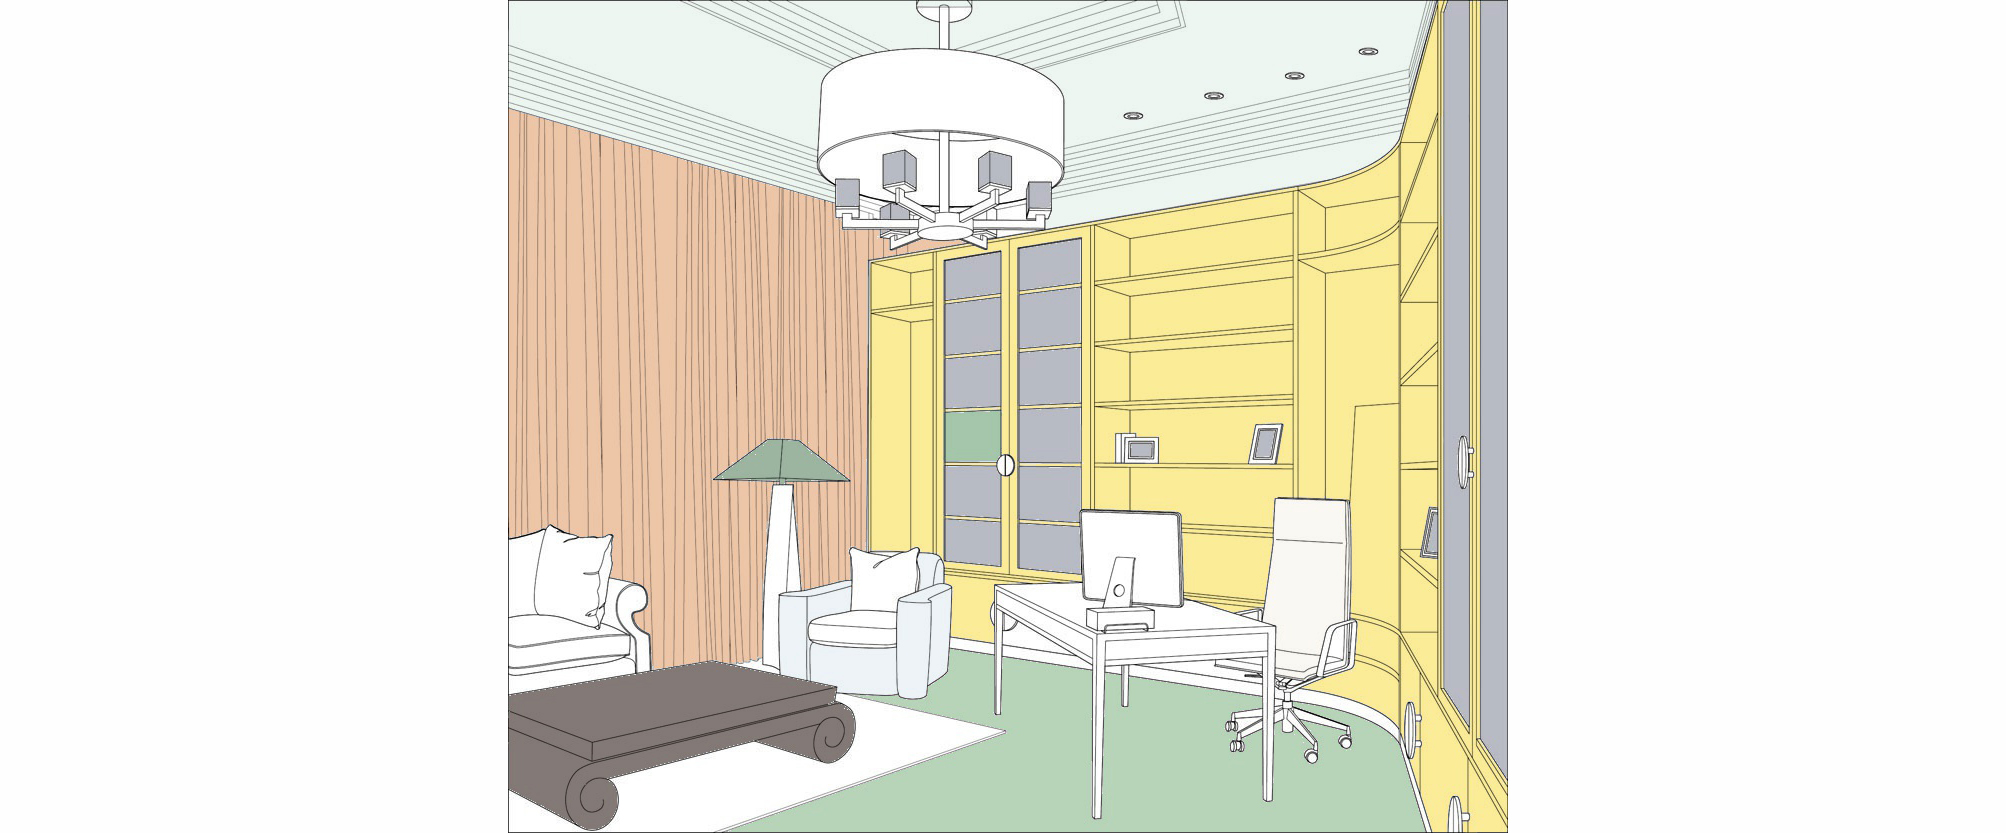
\includegraphics[width=\linewidth,keepaspectratio]{data/chapter-4/快乐儿童3.jpg}
\caption{输入“快乐的儿童”}
\label{figure:儿童2}
\end{figure}



\section{效果图类型的测试案例}

本系统的色彩方案可以用于室内设计、服装设计、产品设计、平面设计、交互视觉设计等。但是上色预览的算法并不适用于每种工作。系统准备了室内设计,服装设计各1套效果图线稿预览,之测试发现,如图~\ref{figure:温柔_IandF},对于上色区域占图片比例较小并且色彩有限的服装、产品效果图本系统也可以使用,但系统效果更适合室内设计效果图。

\begin{figure}[!htbp]
\centering
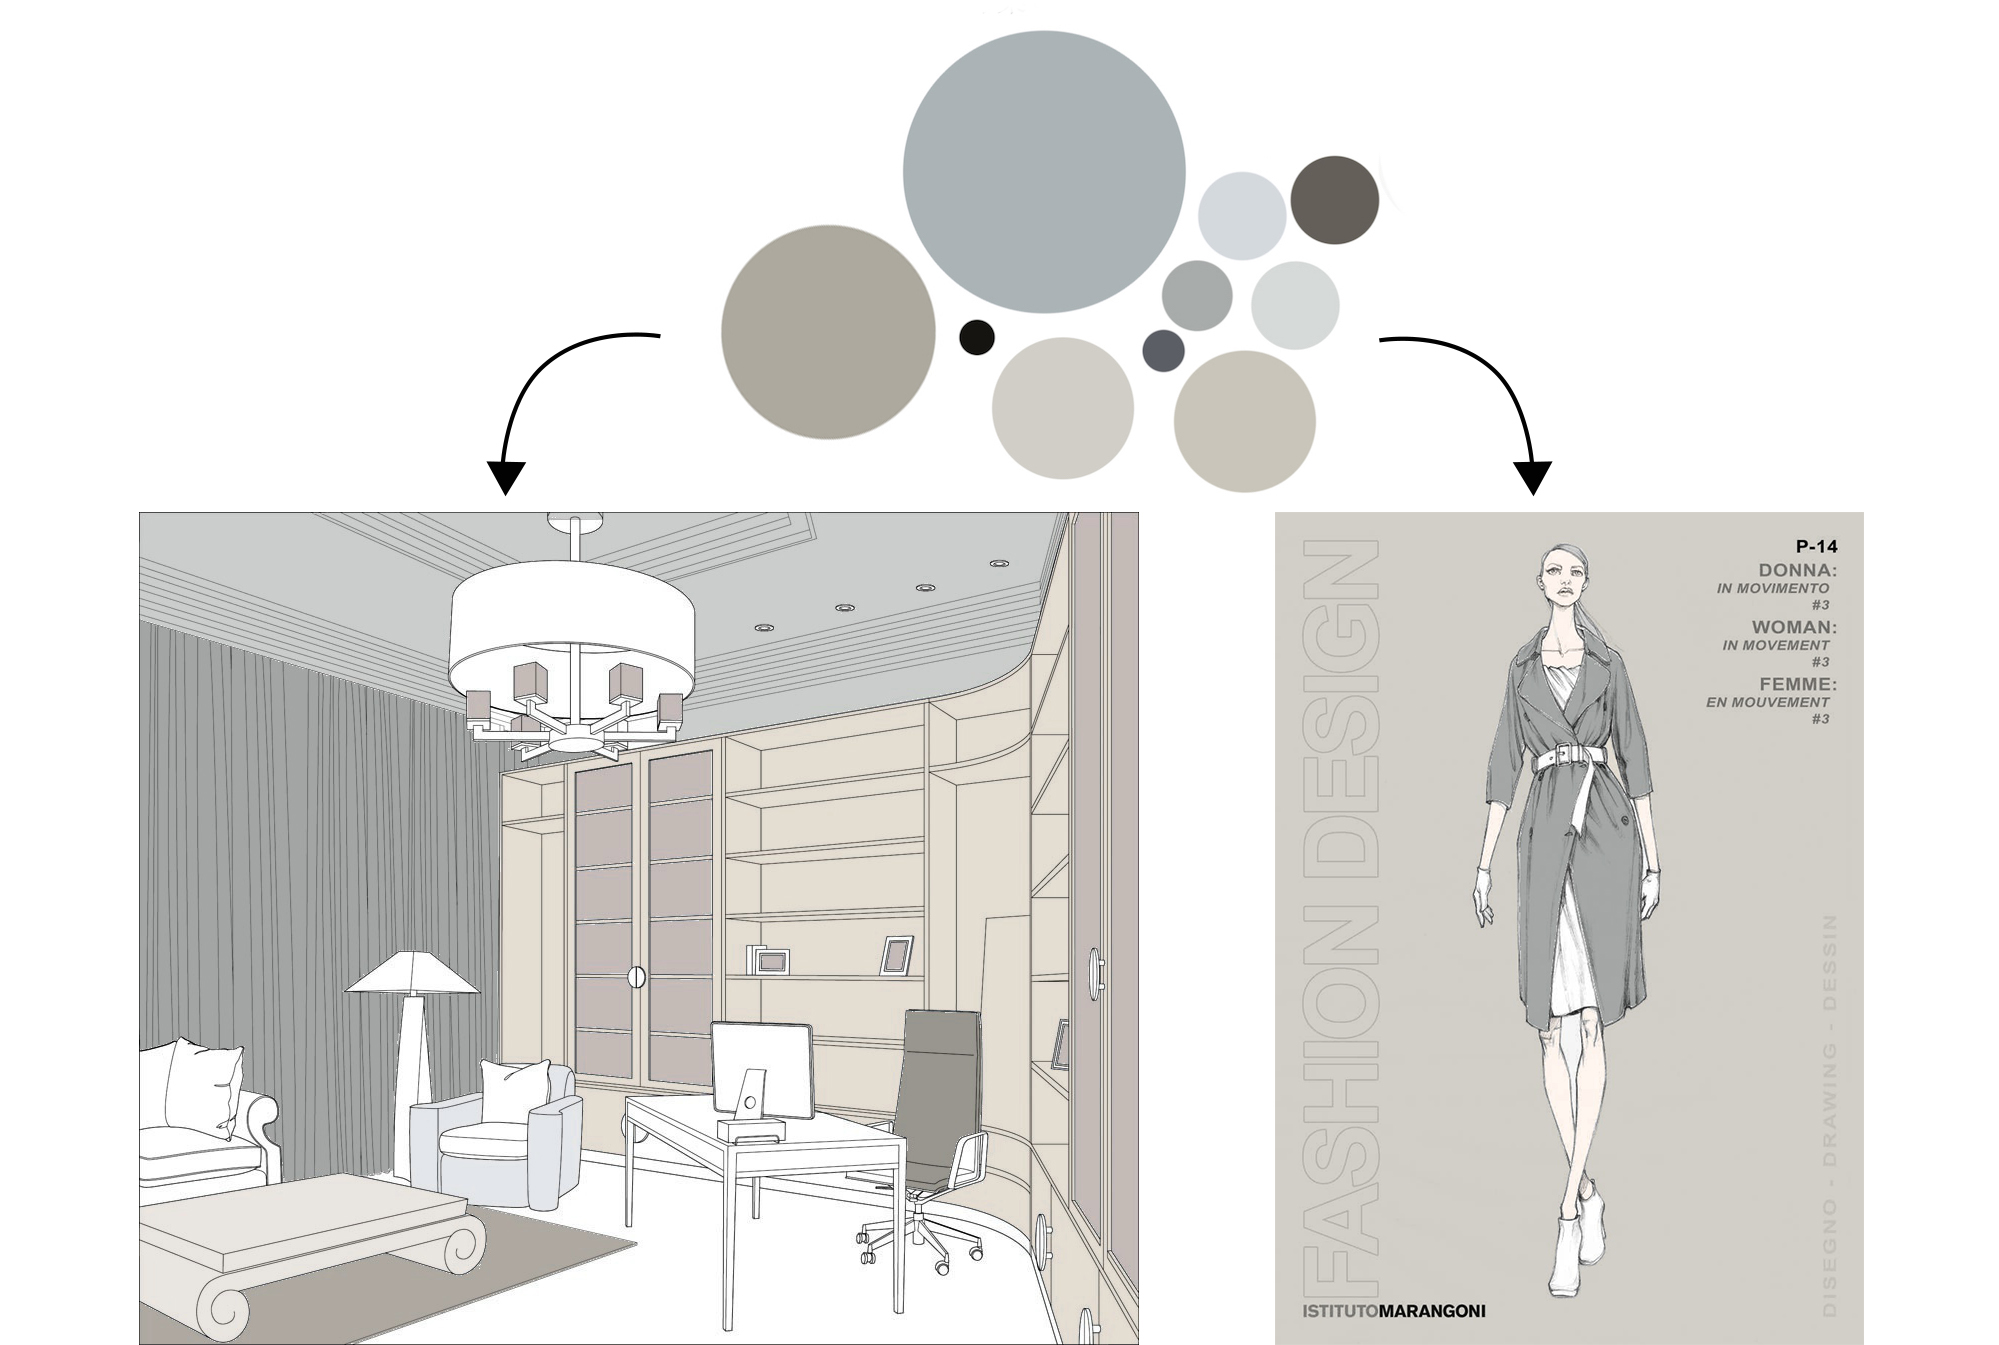
\includegraphics[width=\linewidth,keepaspectratio]{data/chapter-4/温柔_IandF.jpg}
\caption{色彩方案:“温柔”对室内设计和服装设计效果图的预览}
\label{figure:温柔_IandF}
\end{figure}

配色方案对于服装设计是适用的,然而由于服装设计效果图有一些特点,首先服饰在整个图片上的面积较小,填充算法的种子点行走到服装上到几率较小,如果是有花纹的服装,花纹的色彩连续性无法保证,小的配饰更难以填充,所以本系统的上色算法更适合室内设计。

对于其他的效果图,可以使用具体匹配的上色方式。对于产品设计效果图,每个产品上的出现颜色不多,可能有成套的不同颜色的产品,更适合简单的标注上色预览。而对于网站视觉设计等,网页的框架往往预先设定比例和模式,使用堆栈的方式上色是非常适合的,在很多的情况下网站设计适用矢量图片,可以直接标注色彩上色。综上,上色方式并不适用某些效果图,但配色方案对于产品设计、网页设计都是适用的,

\section{本章小结}

经过输入语句测试案例,本系统可以对语义精确的响应。对于“冷静的男性化的”房间、“温柔的女性化的”房间、“快乐的儿童的”房间,配色有明显的差别,符合人类的心理预期。而对于“温柔的”和“温柔的女性化的”,这样信息叠加的语句也有相似而差异的配色方案结果。

对于文本不同而意义相同的语义延伸词语,本系统的word embeding模型能够实现同义匹配,并且将其排列在文本完全相同的情况之后搜索到。对于不含有信息的干扰语句,本系统的word embeding模型能够实现信息提取,和不含有干扰语句的情况下得到的结果差别很小。对于含有并列信息的输入语句,搜索的结果受到艺术品数据库的限制,不一定存在完全符合所有并列信息的艺术品文本,所以搜索到的文本结果分为偏向各信息的内容,使用交互的方式来解决这各限制带来的偏差。

对于效果图的类型,本系统的色彩可以用于室内设计、服装设计、产品设计、平面设计、交互视觉设计等。但是上色预览的算法并不适用于每种工作,本系统的上色算法更适合室内设计效果图。对于产品设计、网页设计、服装设计等工作,可以使用各自匹配的上色预览算法。







